\chapter{Implementing the filters} % Main chapter title
\label{Chapter6ImplementingFilters} % For referencing the chapter elsewhere, use \ref{Chapter1Introduction}
\lhead{\emph{Implementation}} % This is for the header on each page - perhaps a shortened title

%----------------------------------------------------------------------------------------

We will cover now the results of the main development phase of the project, concerning the implementation of the MOA privacy preserving filters and the design decisions taken for each of them.

\section{Alternatives exploration}
\label{Implementation:Alternatives}

The Massive Online Analysis stream mining framework is built in the Java language, thus providing some benefits in terms of portability, ease of maintenance and development, but also exposing some drawbacks, mainly due to the lack of easily parallelizable code, like is the case with C or Fortran by using the OpenMP\footnote{OpenMP (Open Multi-Processing) is a programming interface that supports multi-platform shared memory multiprocessing programming in C, C++, and Fortran. It consists of a set of compiler directives, library routines, and environment variables that influence run-time behavior.~\citep{web:Wiki:OpenMP}} language extensions. Given the language enforcement MOA imposes and the existence of well-known SDC toolsuites, like the \texttt{sdcMicro} R package (reviewed in~\sref{State::SDC::sdcMicro}), an analysis of possible alternatives was taken during the first weeks of the project's development phase.

\subsection{\texttt{sdcMicro} \& Java}
\label{Implementation:Alternatives:sdcmicro}

The most direct alternative, besides actually implementing the filters, was to use the \texttt{sdcMicro} library to perform the necessary calculations over the streaming data originated in MOA and take the results back to the framework. This approach can be better understood in~\fref{fig:ppsm-R}: a bi-directional connection between the Java runtime (the Java Virtual Machine or JVM) and the R process would be needed to be able to use the SDC methods of the \texttt{sdcMicro} library. The results of the exploratory analysis of this type of solution are summarized in~\tref{table:JRI-pros-cons}.

\begin{figure}[h]
	\centering
	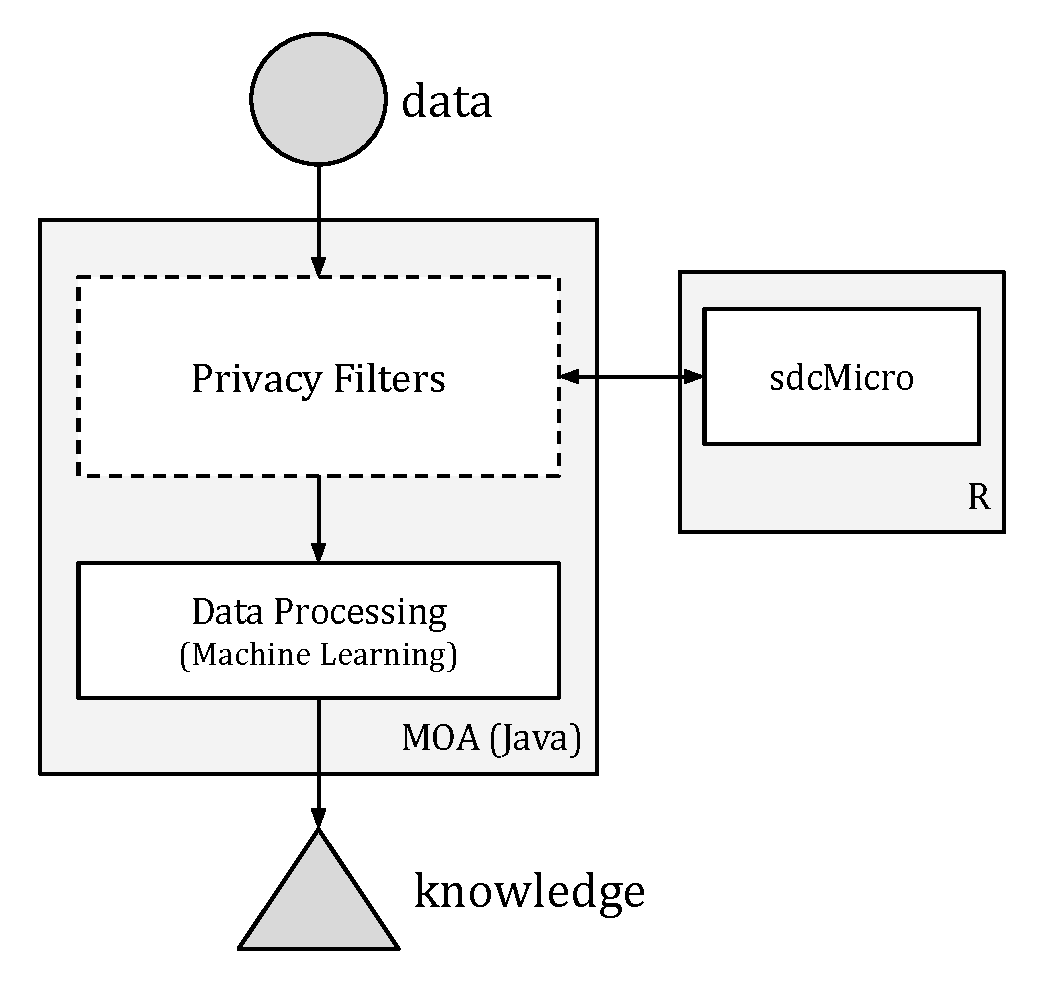
\includegraphics[width=0.6\textwidth]{figures/moa-ppsm-R.pdf}
	\caption{R/Java hybrid solution using the \texttt{sdcMicro} package.}
	\label{fig:ppsm-R}
\end{figure}

This interconnection could be achieved by using some existing technologies that perform the inter-process communication based on different approaches:

\begin{itemize}
	\item
	\textbf{rJava/JRI:} the \texttt{rJava} and \texttt{JRI} counterparts are a couple of libraries designed to provide low-level communication between the Java Virtual Machine (JVM) and an R process. \texttt{rJava} provides a low-level bridge between R and Java via the Java Native Interface (JNI)\footnote{The Java Native Interface is a standard programming interface for writing Java native methods and embedding the Java Virtual Machine into native applications. The primary goal is binary compatibility of native method libraries across all Java virtual machine implementations on a given platform~\citep{web:Oracle:JNI}.}. It allows to create objects, call methods and access fields of Java objects from R~\citep{web:rJava}. On the other side, \texttt{JRI} is a Java/R Interface, which allows to run R inside Java applications as a single thread. Basically, it loads R dynamic library into Java and provides a Java API to R functionality~\citep{web:JRI}.
	
	\item
	\textbf{Rserve:} it is a TCP/IP server which allows other programs to use facilities of R from various languages without the need to initialize R or link against an R library. A typical use is to integrate R backend for computation of statstical models, plots etc. in other applications~\citep{web:Rserve}.
\end{itemize}

Due to performance related to networking protocols against native interface communication, \texttt{Rserve} was discarded as an option to implement filters for MOA: a streaming environment requires the maximum throughput possible for its algorithms and, thus, the overhead associated with TCP-based IPC is considered to be excessive.

Anyway, either of such solutions imply that marshalling and unmarshalling techniques would have to be applied, in order to transform the data structures that are differently used by R and Java. Moreover, even though that no SDC algorithm would need to be implemented, the interconnect code would not be easy to maintain.

Finally, there is another important argument against the R/Java hybrid approach: its strong reliance in external dependencies. These dependencies not only make the installation of the SDC-enabled MOA framework more difficult, but are directly linked to third-party software and \textit{system} libraries, making the environment less stable and robust, from the software user point of view. These dependencies are shown in~\fref{fig:ppsm-JRI-arch}

\begin{figure}[h]
	\centering
	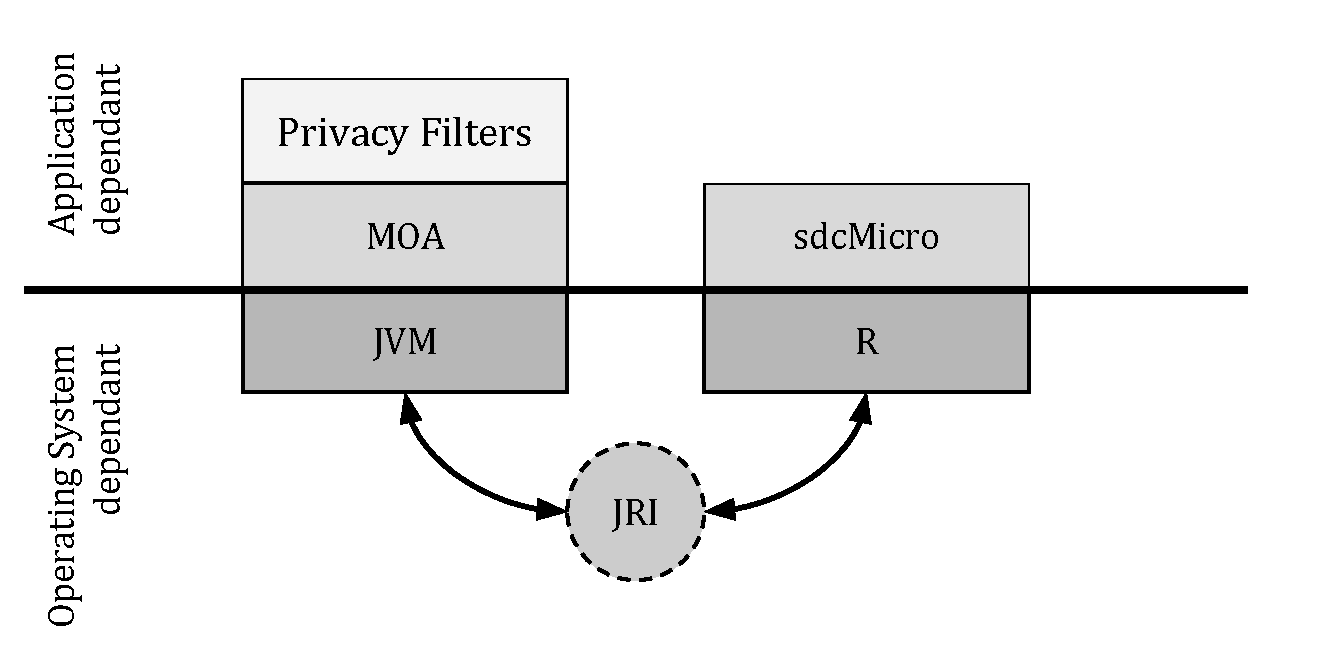
\includegraphics[width=0.8\textwidth]{figures/moa-ppsm-JRI-arch.pdf}
	\caption{JRI based R/Java hybrid solution architechture: strong dependencies.}
	\label{fig:ppsm-JRI-arch}
\end{figure}

\begin{table}
	\centering
	\begin{tabular}{ll}
		\hline
		\textbf{Benefits}     & \textbf{Drawbacks}                     \\ \hline
		Faster development    & No algorithms are indeed developed     \\
		Easily extensible     & Strong dependencies                    \\
		SDC methods are right & Depends on external installed software \\
		                      & Needs system libraries to work         \\
		                      & Maintanability is harder               \\
		                      & Reduced performance due to marshalling \\ \hline
	\end{tabular}
	\caption{Evaluation of the R/Java hybrid solution.}
	\label{table:JRI-pros-cons}
\end{table}

\subsubsection{Renjin}

Yet another altenative was explored that was meant to interconnect MOA with the \texttt{sdcMicro} package: the Renjin project~\citep{web:Renjin}. \textbf{Renjin} is a JVM-based interpreter for the R language: all computations of any R package can be executed upon the JVM, instead of a separate R process. This way, the dependency that this project could have had on R and some system libraries disappeared. However, it is worth noting that, even with Renjin, data structures conversion would have to be performed, rendering its use as impractical as the use of the \texttt{JRI} library. Moreover, the \texttt{sdcMicro} package was still not available in its JVM \textit{port} at the time of the evaluation due to some internal dependencies and errors, and we could not wait for it to be solved.

\subsection{Chosen alternative}

As a simple remark, the final decision was to actually develop the filters for the MOA framework by extending it, in the form of a \textbf{pure Java} implementation.
\section{MOA \& Privacy Filters}
\label{Implementation:PrivacyFilter}

\textbf{Notation:} from now on, a text stylized with a monospaced font like \texttt{this example} will refer to an actual programming artifact: a variable, class, file name, etc.

We have already showed along this report that \textit{filters} are a feature of the MOA framework. Filters are, actually, a particular form of \textit{stream}. Whenever a filter should be applied to a stream to perform a posterior analysis, a \texttt{FilteredStream}\footnote{All documentation of the MOA API can be found on \url{http://www.cs.waikato.ac.nz/~abifet/MOA/API/index.html}} is built. This class takes a generic \texttt{Stream} object as the input stream and a list of \texttt{StreamFilter}s, which are also \texttt{Stream}s, if we examine their type hierarchy. Taking advantage of the existence of both the \texttt{FilteredStream} and \texttt{StreamFilter} classes, we can begin designing the privacy filters that will implement the actual SDC methods.

\subsection{\texttt{PrivacyFilter}}
\label{Implementation:PrivacyFilter:PrivacyFilter}

Thanks to the object-oriented capabilities of the Java language, we can design and implement a generic abstract data type for all proposed SDC algorithms. By doing so, we will be able to centralize some of the common logic behind them. The abstract type of the privacy filters is the \texttt{PrivacyFilter} class. An incomplete UML diagram of the specification of this class and its most relevant parent types can be seen in~\fref{fig:privacy-filter-uml}.

Concerning the responsibility\footnote{In object-oriented programming, the \textit{single responsibility principle} states that every class should have responsibility over a single part of the functionality provided by the software, and that responsibility should be entirely encapsulated by the class (\citet{web:SOLID}).} of this class, there is a main task that the \texttt{PrivacyFilter} is meant to address: the measurement or \textit{evaluation} of the \textbf{disclosure risk} (DR) and the \textbf{information loss} (IL). The approach is to let the SDC method (the \textit{concrete} subclass) anonymize the \textit{instances}\footnote{In the MOA context, records in a dataset (in a stream) are called \textit{instances} and are represented using the \texttt{Instance} interface.} of the stream and collect them, along with the original instances that have been processed. The evaluation of both magnitudes, DR and IL, is performed by \textit{estimators} using these \textit{pairs} of instances (see Estimators, below). The mechanism is best understood with the schematic presented in~\fref{fig:privacy-filter-schematic}.

\begin{figure}[h]
	\centering
	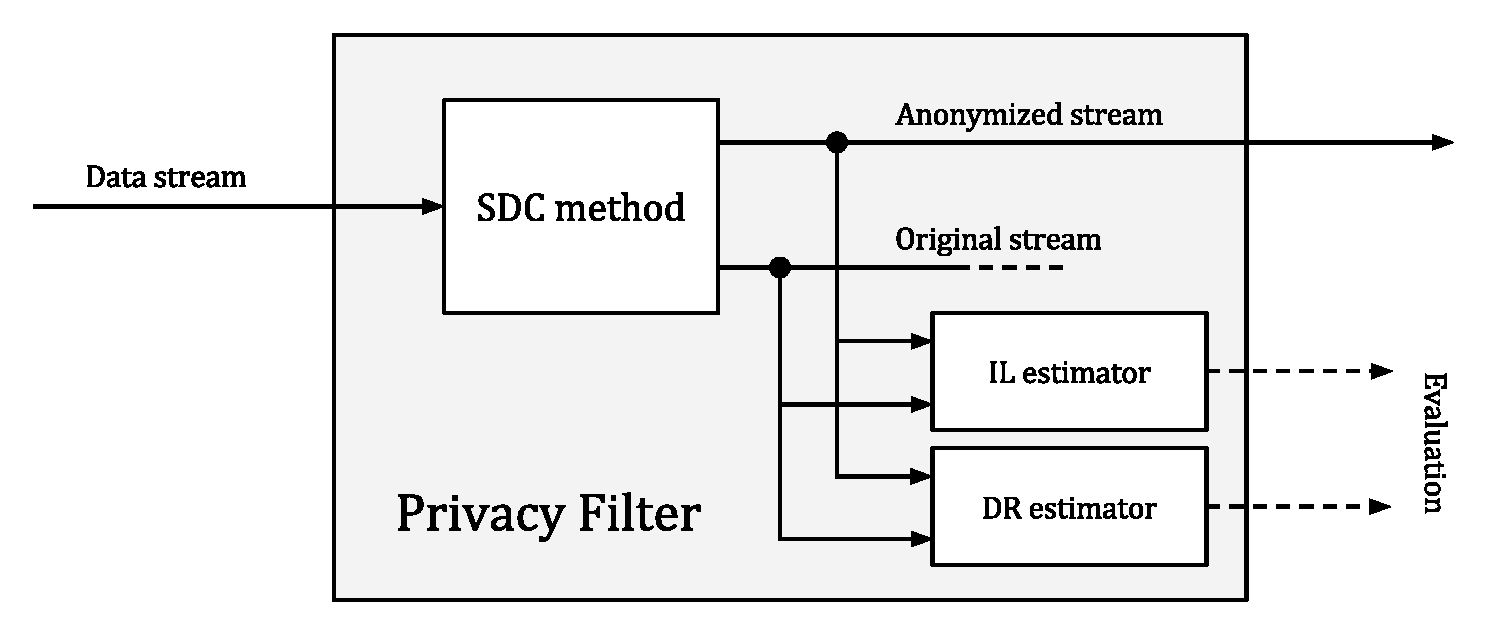
\includegraphics[width=0.8\textwidth]{figures/privacy-filter-schematic.pdf}
	\caption[\texttt{PrivacyFilter} data flow schematic.]{A schematic of the tasks performed by the \texttt{PrivacyFilter} class, showing the stream data flow.}
	\label{fig:privacy-filter-schematic}
\end{figure}

\subsubsection*{Implementation details}
\label{Implementation:PrivacyFilter:PrivacyFilter:Details}

The \texttt{PrivacyFilter} class is, by construction, an \texttt{InstanceStream} and a \texttt{StreamFilter} (see~\fref{fig:privacy-filter-uml}) but also, and most importantly, an \texttt{AnonymizationFilter}. This last \textit{interface}, which the \texttt{PrivacyFilter} implements, allows to encapsulate all privacy-preserving behaviour in a single module.

The most important of the methods defined in the \texttt{AnonymizationFilter} type is

\begin{center}
	\texttt{nextAnonymizedInstancePair() : InstancePair}
\end{center}

which is left to be implemented (it is \textit{abstract} at the \texttt{PrivacyFilter} level) by any subclass. This way, we can use \textit{inversion of control}\footnote{The \textit{Hollywood principle} or \textit{inversion of control} pattern is a software design methodology that takes its name from the cliché response given to amateurs auditioning in Hollywood: "Don't call us, we'll call you". It is a useful paradigm that assists in the development of code with high cohesion and low coupling that is easier to debug, maintain and test.} to force a subtype define the concrete behaviour of the function, while still conforming to a precise \textit{contract}. The \texttt{InstancePair} returned by this abstract method is just a \textit{pair} structure containing both the original and anonymized instances that should be streamed next. If we say that $x$ is an instance and $x'$ its anonymized counterpart, the \texttt{InstancePair} class would simply be the tuple $\langle x, x' \rangle$.

\begin{figure}[h]
	\centering
	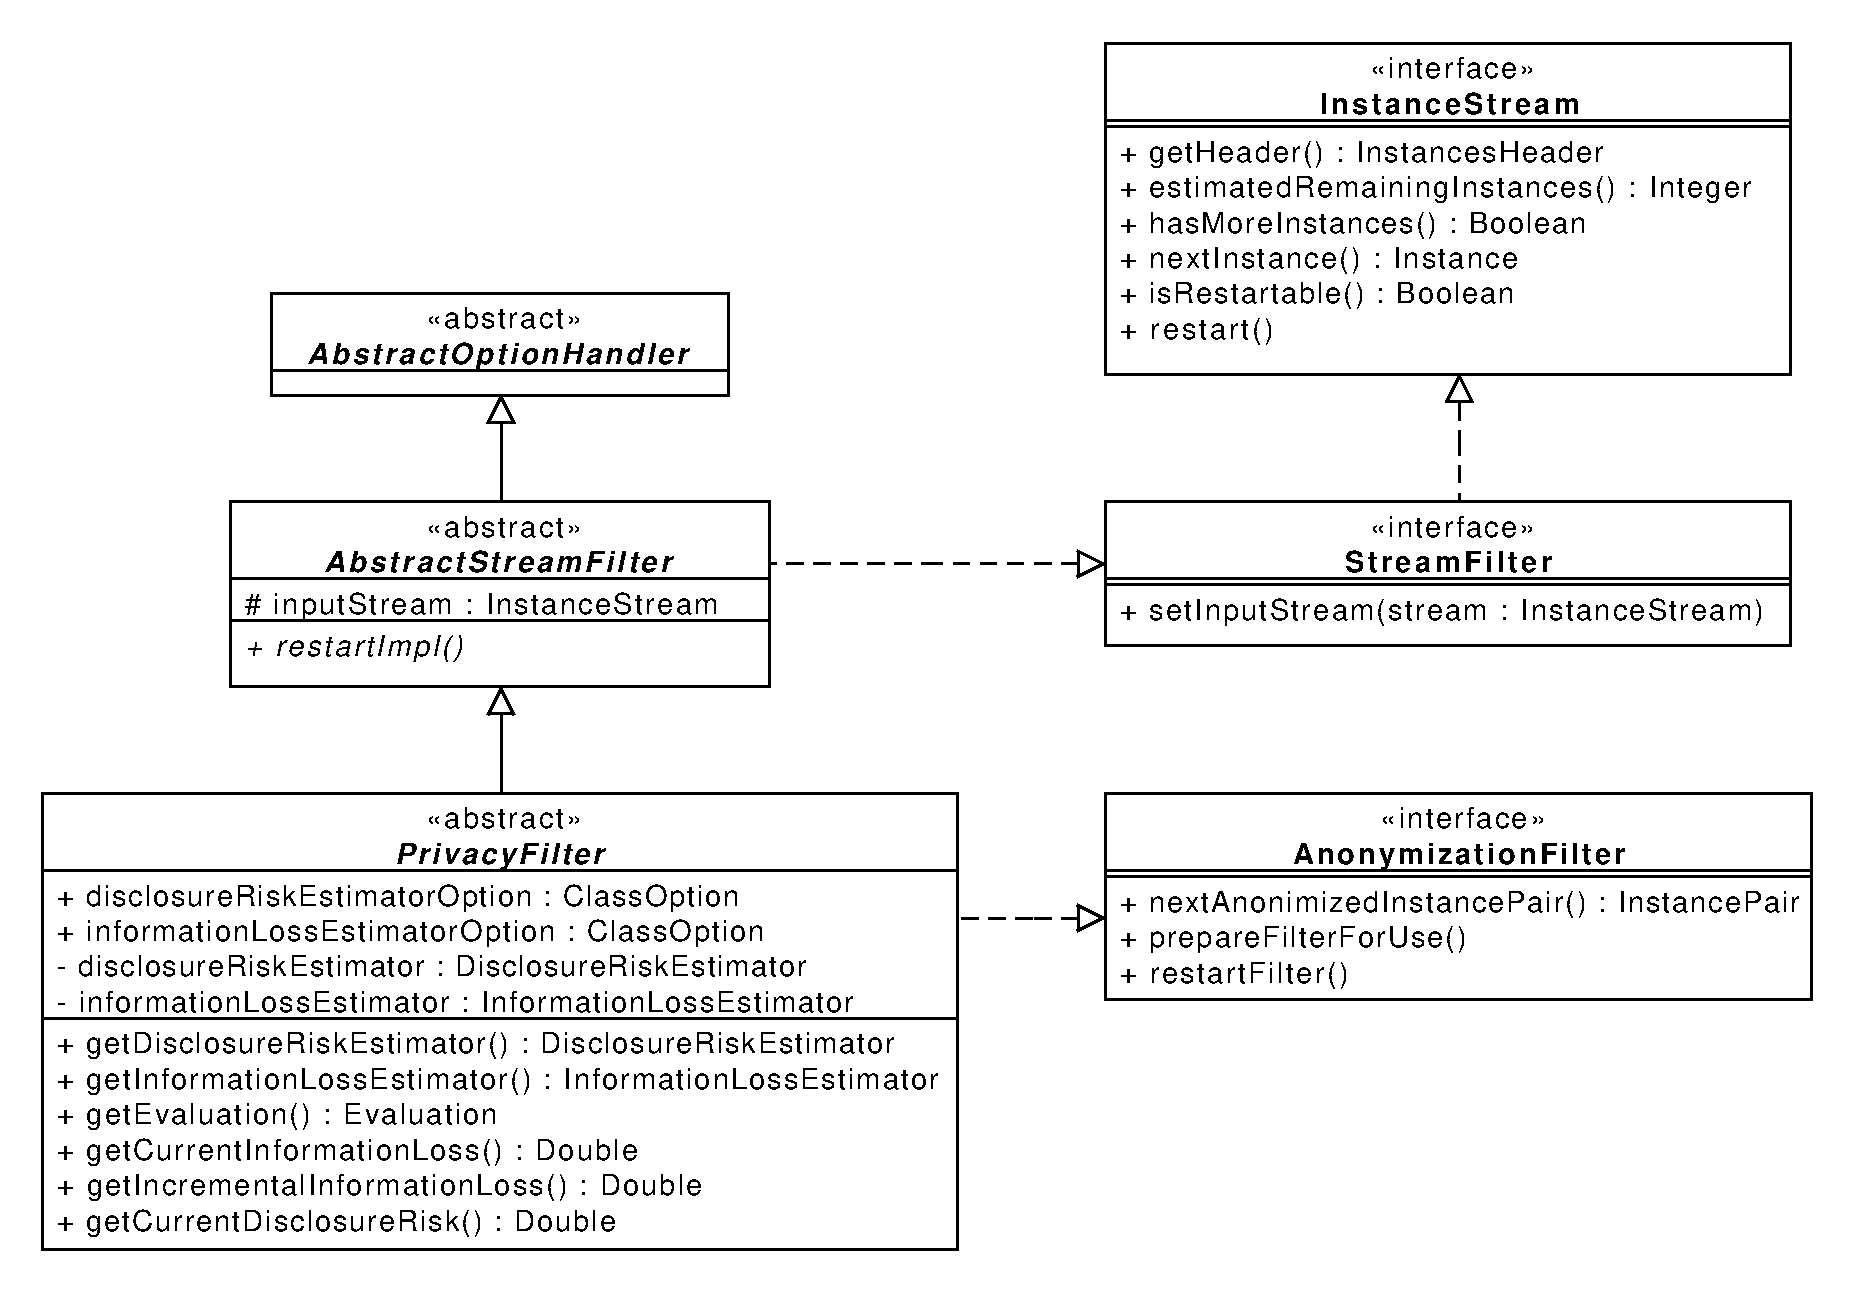
\includegraphics[width=1.0\textwidth]{figures/class_PrivacyFilter.pdf}
	\caption[\texttt{PrivacyFilter} type hierarchy diagram.]{UML class diagram of the relevant types in the \texttt{PrivacyFilter} class hierarchy. Notice that not all the involved types are shown.}
	\label{fig:privacy-filter-uml}
\end{figure}

\subsubsection*{Estimators}
\label{Implementation:PrivacyFilter:PrivacyFilter:Estimators}

The estimators used by the \texttt{PrivacyFilter} class are desgined to be modular and, most of all, easily modifiable: they are just interfaces defining a contract that all estimators must implement. The methods belonging to such contracts can be seen in~\fref{fig:estimators-uml} (the concrete estimators implementation is explained in~\sref{Implementation:Estimators}). Again, there is one particular method that is most important in the estimators context:

\begin{center}
\texttt{performEstimationForInstances(instancePair : InstancePair)}
\end{center}

This method is the generic way for the \texttt{PrivacyFilter} to feed the estimators with $\langle x, x' \rangle$ tuples (\texttt{InstancePair}s). The estimators have the responsibility of performing the necessary calculations using this stream of pairs of instances.

\begin{figure}[h]
	\centering
	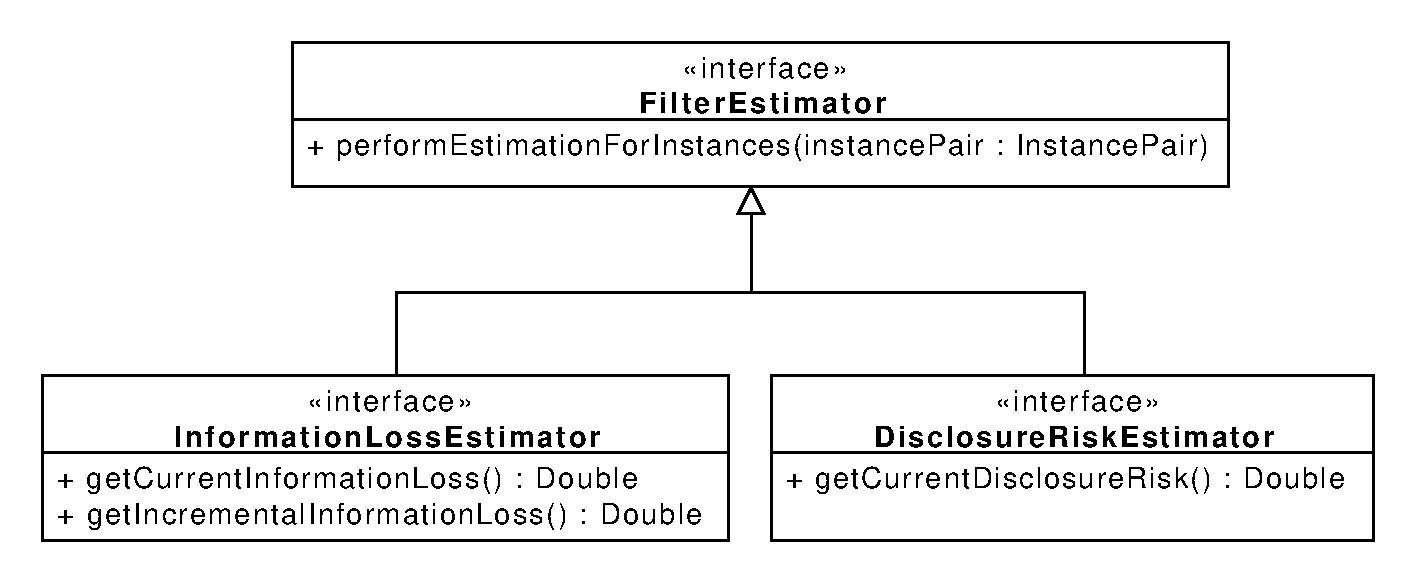
\includegraphics[width=0.8\textwidth]{figures/class_Estimators.pdf}
	\caption[\texttt{FilterEstimator} type hierarchy diagram.]{Class diagram of the \texttt{FilterEstimator} type hierarchy.}
	\label{fig:estimators-uml}
\end{figure}

Finally, the DR and IL estimators used by a \texttt{PrivacyFilter} can be configured at runtime by setting the appropriate \textit{options}\footnote{The MOA framework makes extensive use of configurable \textit{options}, which can be set either on a command line execution or via the GUI that MOA provides.} of the filter.

\subsection{Filters ecosystem}
\label{Implementation:PrivacyFilter:Ecosystem}

Having reviewed the basic \texttt{PrivacyFilter} generic type, we can now provide a couple of figures that introduce the final structure of the privacy filters class ecosystem. The \textit{package} encapsulation of the methods can be seen on~\fref{fig:moa-ppsm-packages}. An incomplete\footnote{Most of the classes shown in the diagram depend on others for their internal implementation, but, for the sake of concreteness, they are not shown, as are not relevant for the purpose of this report.} class diagram of the filters is shown in~\fref{fig:moa-ppsm-class-uml}.

\begin{figure}
	\centering
	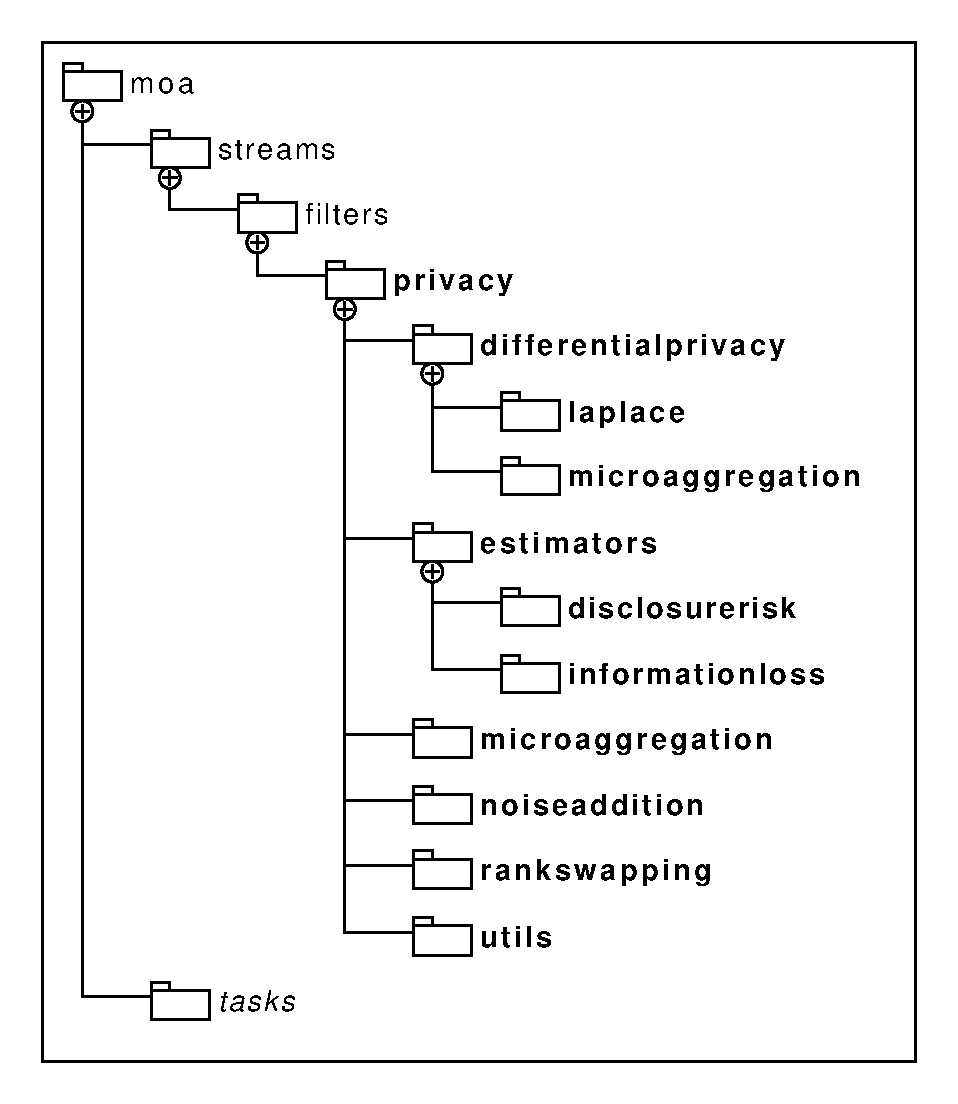
\includegraphics[width=0.5\textwidth]{figures/moa-ppsm-packages.pdf}
	\caption[Package diagram of the privacy filters ecosystem.]{Package organization of the privacy filters. \textbf{New} packages (not existing in the MOA framework) are shown in bold. \textit{Existing} packages that have been extended with new types are shown in italics.}
	\label{fig:moa-ppsm-packages}
\end{figure}

\begin{figure}
	\centering
	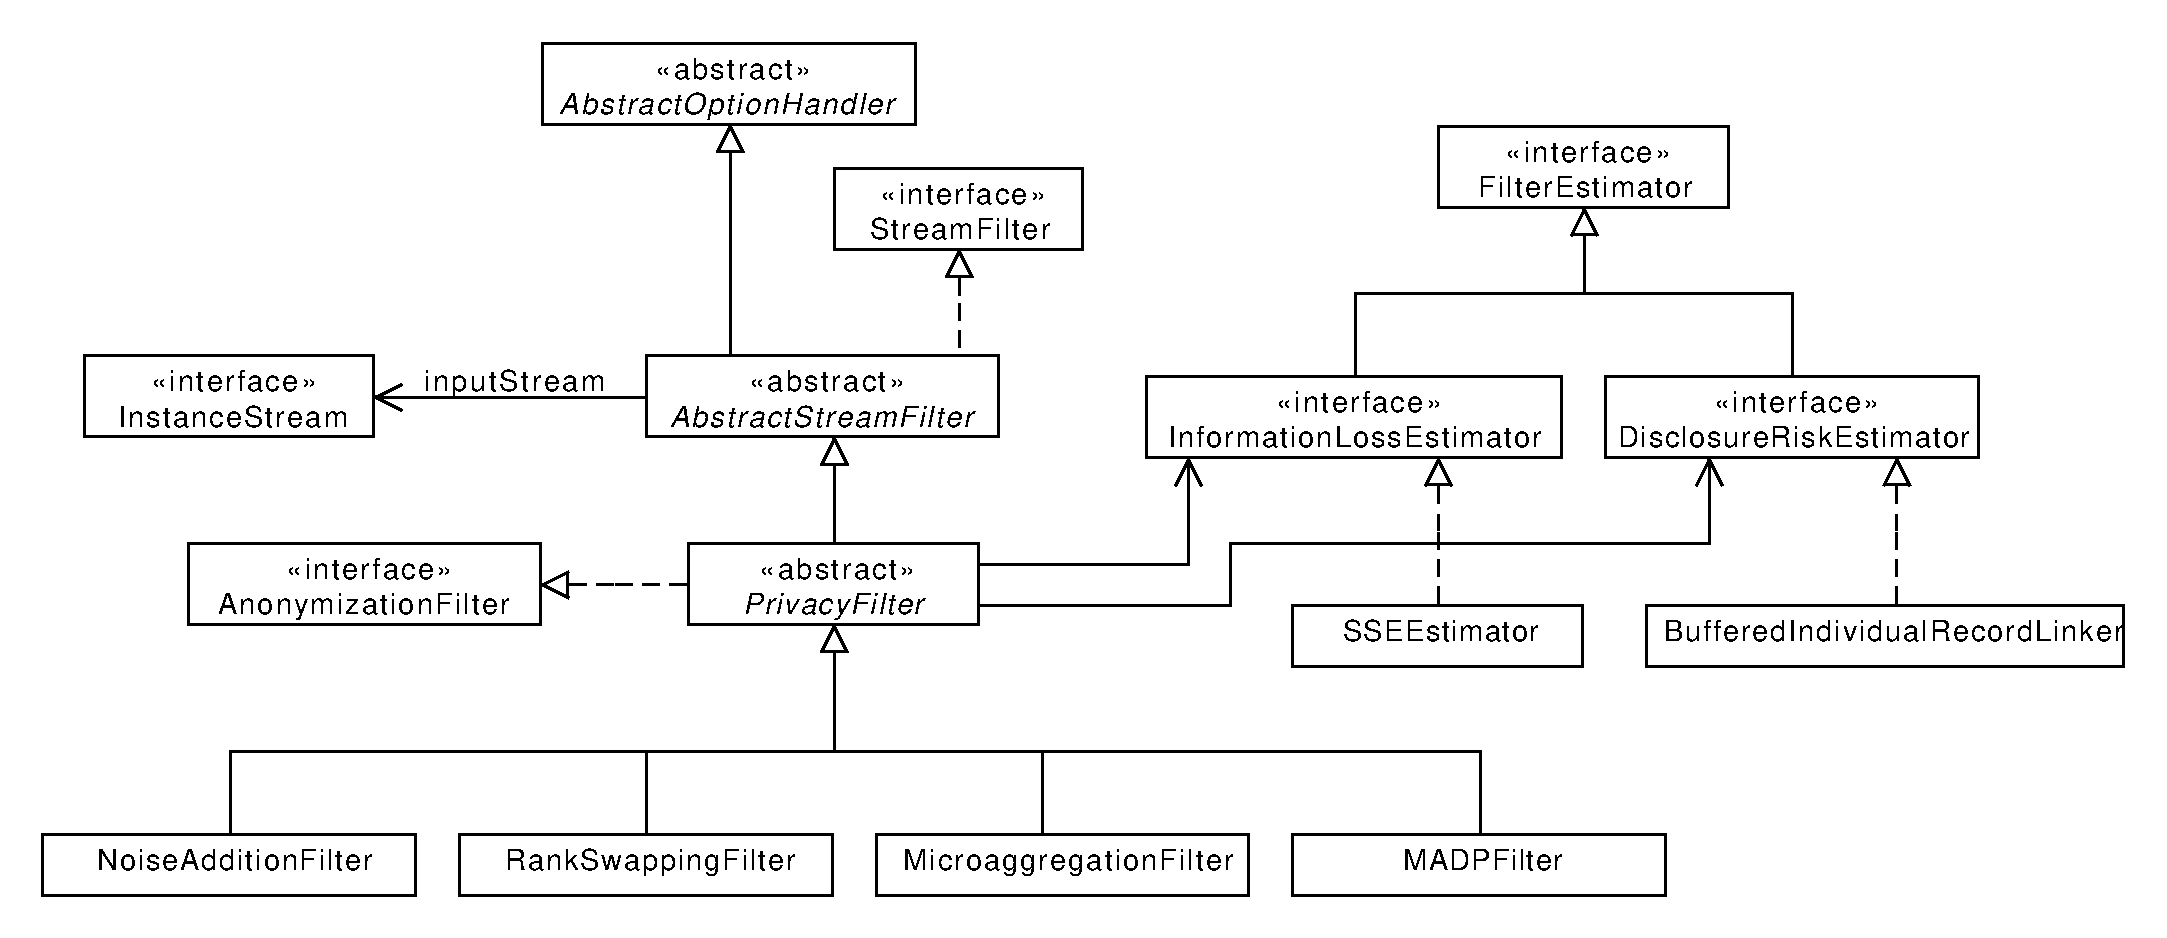
\includegraphics[width=1.0\textwidth]{figures/refactored-ppsm-class-diagram.pdf}
	\caption[Class diagram of the privacy filters ecosystem.]{Class diagram of the privacy filters ecosystem. Only the relevant types are shown and no method or member specifications have been included.}
	\label{fig:moa-ppsm-class-uml}
\end{figure}
\section{Estimators}
\label{Implementation:Estimators}

\subsection{\texttt{BufferedIndividualRecordLinker}}
\label{Implementation:Deployment:RecordLinker}

\subsection{\texttt{SSEEstimator}}
\label{Implementation:Deployment:SSE}
\section{\texttt{NoiseAdditionFilter}}
\label{Implementation:NoiseAddition}

\subsection{Design}
\label{Implementation:NoiseAddition:Design}

\subsection{Implementation details}
\label{Implementation:NoiseAddition:Details}

\section{\texttt{MicroaggregationFilter}}
\label{Implementation:Microaggregation}

\subsection{Design}
\label{Implementation:Microaggregation:Design}

\subsection{Implementation details}
\label{Implementation:Microaggregation:Details}

\section{\texttt{RankSwappingFilter}}
\label{Implementation:RankSwapping}

The rank swapping SDC method described in~\sref{Theory:SDCMethods:RankSwapping} is implemented by the \texttt{RankSwappingFilter} class. We must notice that it is a very naïve implementation and certainly not the fastest of the filters. As we will discuss later, future work is needed to enhance the performance of this filter.

\subsection{Design}
\label{Implementation:RankSwapping:Design}

The \texttt{RankSwappingFilter} is the second \textit{buffered filter} that has been implemented in this project (see~\sref{Implementation:BufferedFilter}). Almost the same data structures (the $W$, $W'$ and $A$ buffers) used by the \texttt{MicroAggregationFilter} are used by the rank swapping algorithm. The main difference with respect to the microaggregation algorithm is that the set $A$, used to know whether or not an \textit{instance} has already been anonymized, is now used to know whether or not a \textit{value} $w_{ij}'$ (this is, the $j$-th attribute value of the $i$-th instance in $W'$) has been \textit{swapped} or not. Summarizing, we say that $w_{ij}'$ has been swapped if $w_{ij}' \in A$.

\begin{figure}
\centering
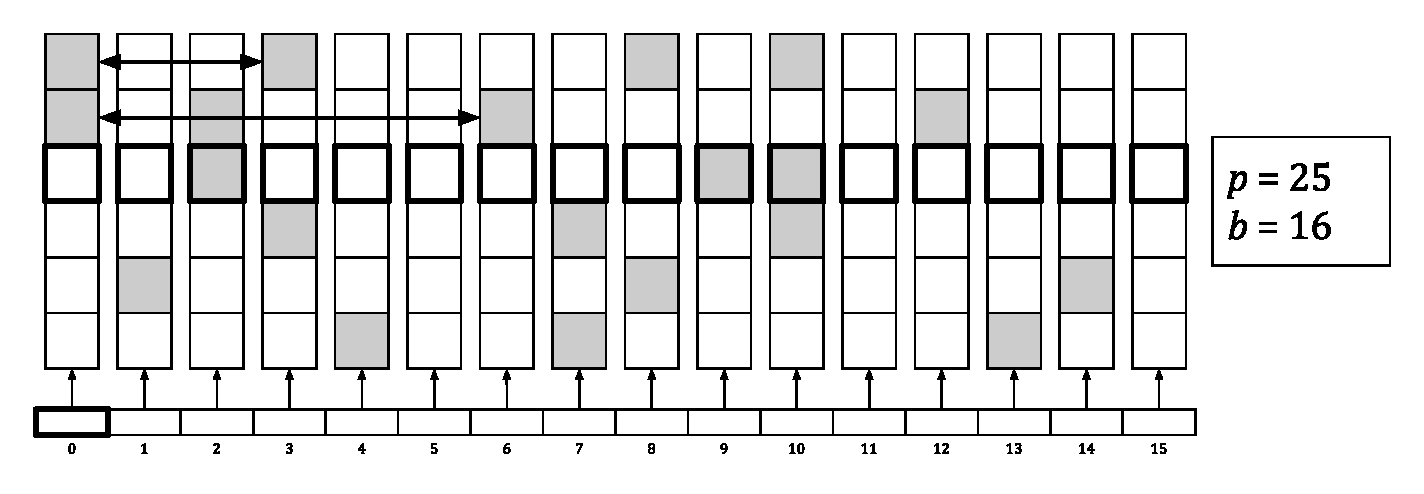
\includegraphics[width=1.0\linewidth]{figures/rank-swapping-schematic-1.pdf}
\caption[Rank swapping algorithm schematic.]{Rank swapping algorithm schematic. Two attributes of the target record (position 0) have already been \textit{rank swapped} with other values from instances in the buffer. The variable being now processed is highlighted.}
\end{figure}

\begin{figure}
\centering
\makebox[\textwidth][c]{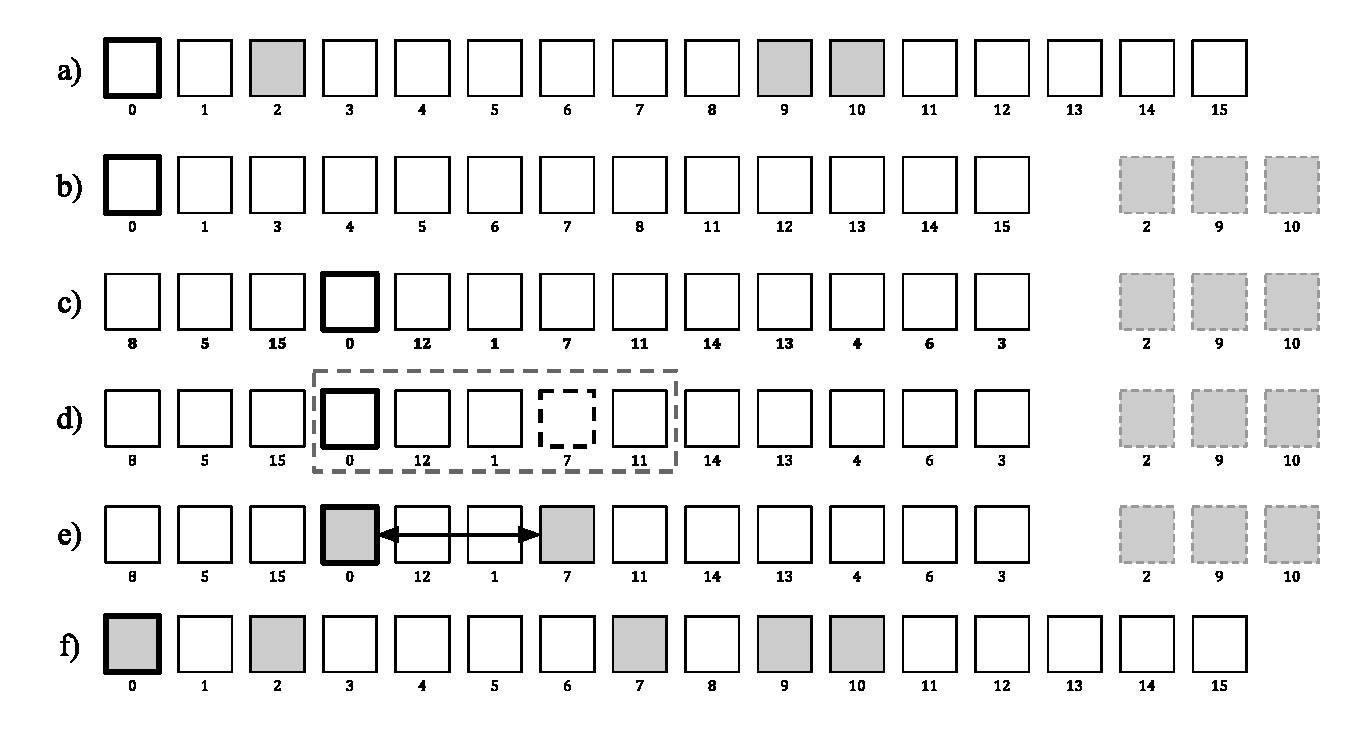
\includegraphics[width=1.1\linewidth]{figures/rank-swapping-schematic-2.pdf}}
\caption[Rank swap of an attribute.]{Rank swap of a single attribute for a target instance $\tau$. First, the non already swapped values of the attribute are filtered from the instances in the buffer $W$ (b) and are ranked, i.e., sorted (c). A maximum swap range is calculated using the $p$ parameter (d) and a value within this range is selected to perform the swap (e). Finally, the vector of values is returned in the original order they were in the buffer (f).}
\label{fig:rank-swapping-schematic-2}
\end{figure}

The design of this SDC method follows almost exactly the explanation given in the theoretical background chapter (\sref{Theory:SDCMethods:RankSwapping}): for each instance processed from the stream, values of each variable $j$ are ranked in ascending order, this is, they are \textit{sorted}. Each ranked value is then swapped with another ranked value, randomly chosen within a restricted range, controlled by the input parameter $p$, which denotes that swapped values cannot differ more than $p\%$ of the total number of records. A more formal description of its implementation is given in~\alref{al:rank-swapping}, along with its auxiliar procedure \texttt{selectSwap()} (see~\procref{al:select-swap}). Also, a more visual explanation is shown in~\fref{fig:rank-swapping-schematic-2}.

\begin{algorithm}[H]
\KwData{$W', A, p$}
\KwResult{the target instance $\tau$ is anonymized}
\Begin{
	$\tau \leftarrow w_0'$\;
	\For{$j \in \mathrm{attributes}(\tau)$}{
		$\gamma \leftarrow \mathrm{selectSwap}(W',p,j)$\;
		$\sigma \leftarrow w_\gamma'$\;
		$\mathrm{swap}(\tau_j, \sigma_j)$\;
		$A \leftarrow A \cup \tau_j \cup \sigma_j$\;
	}
}
\caption{Rank Swapping\label{al:rank-swapping}}
\end{algorithm}

\begin{procedure}
\KwData{$W'$ buffer, $p$ parameter and $j$ attribute}
\KwResult{the index $\gamma$ of the instance with which the swap will be done}
\Begin{
	$V \leftarrow \mathrm{Vector}(\{\langle w_{ij}', i \rangle~\vert~0 \leq i \leq b-1,~w_{ij}' \notin A\})$\;
	\tcp{Notice that, by construction, $\langle \tau_j, 0\rangle \in V$}
	$V^* \leftarrow \mathrm{sort}(V)$ \tcp{sort by \textit{value}, not by index}
	$t \leftarrow V^*.index(\langle \tau_j, 0\rangle)$\;
	$r \leftarrow 1 + \mathrm{Random}.uniform()~\mathrm{mod}~(p \cdot b~/~100)$ \tcp{$r \in [1, p\% \cdot b] $}
	$s \leftarrow 0$\;
	\eIf{$t + r < V^*.size() $}{
		$s \leftarrow t + r$\;
	}{
		$s \leftarrow V^*.size() - 1$\;
	}
	\tcp{$s$ is the index of the selected value-index pair to be swapped}
	$\langle \cdot,\gamma \rangle \leftarrow V^*[s]$\;
	\KwRet{$\gamma$}\;
}
\caption{selectSwap($W',p,j$)\label{al:select-swap}}
\end{procedure}

If we examine the previous rank swapping algorithm in detail, we can estimate its computational complexity. The cost of swapping a value of an attribute is, basically, that of sorting all of its values: $O(b \cdot \mathrm{log}(b))$, where $b$ is the size of the buffers $W$ and $W'$. Each of the $n$ instances of the stream will have its $m$ attributes rank swapped with those of another record; therefore, the total complexity of the algorithm can be approximated to be $O(n \cdot m \cdot b \cdot \mathrm{log}(b))$.

\subsection{Summary}
\label{Implementation:RankSwapping:Summary}

The \texttt{RankSwappingFilter} class implements rank swapping algorithm to anonymize streaming data by exchanging values of the same attribute between close instances.~\tref{table:rankswapping-summary} summarizes the main properties of this SDC method.

\begin{table}[h]
	\centering
	\begin{tabular}{@{}ll@{}}
	\toprule
	\multicolumn{2}{l}{\textbf{RankSwappingFilter}}                             \\ \midrule
	\textbf{Parameters}   & $p$ (maximum swap range, as a percentage of the buffer size), $b$ (buffer size) \\
	\textbf{Type of data} & Heterogeneous (both numeric and categorical attributes) \\
	\textbf{Cost}         & $O(n \cdot m \cdot b \cdot \mathrm{log}(b))$  \\ \bottomrule
	\end{tabular}
	\caption{\texttt{RankSwappingFilter} summary.}
	\label{table:rankswapping-summary}
\end{table}
\section{\texttt{DifferentialPrivacyFilter}}
\label{Implementation:DifferentialPrivacy}

The concept of \textit{differential privacy} is introduced in~\sref{Theory:SDC:Guarantees:DifferentialPrivacy} and on~\sref{Theory:SDCMethods:LaplaceMechanism} a data release \textit{mechanism} that achieves this privacy guarantee is described: the Laplace mechanism. The drawback of differential privacy is that its definition relies on an interactive \textit{query-response} environment, which is definitely not the one we encounter in stream data mining. However, we can find in the literature some efforts to bring differential privacy to non-interactive settings, such as in~\citet{Leoni:NonInteractiveDiffPriv} and~\citet{Domingo:EnhancingDiffPrivMicroaggregation}. The \texttt{DifferentialPrivacyFilter} is devised to provide a differentialy private release method in such a setting, namely, in the context of MOA privacy filters.

\subsection{Design}
\label{Implementation:DifferentialPrivacy:Design}

Following the idea presented in~\citet{Domingo:EnhancingDiffPrivMicroaggregation}, we have built an SDC method which combines microaggregation with the Laplace mechanism. We recall now the definition of this mechanism:

\begin{definition}~(Laplace mechanisnm)\\
Given a dataset $X$ and a function $f : X \rightarrow \mathbb{R}^d$, with $w \in \mathbb{N}^+$, an $\varepsilon$-differential privacy mechanism $\mathcal{M}$ for releasing $f$ is to publish
\begin{equation*}
\mathcal{M}(X) = f(X) + L
\end{equation*}
where $L$ is a vector of $d$ random variables each drawn from a Laplace distribution $Lap(0,\frac{\Delta(f)}{\varepsilon})$.
\end{definition}

We must remember that the amount of noise introduced by the addition of $L$ to the application of $f$ depends on the \textit{sensitivity} of $f$, denoted by $\Delta (f)$, this is, the maximum variation in the result of $f$ when computed over two neighbour datasets, i.e., sets differing in at most one record. For a fixed $\varepsilon$, the higher the sensitivity of $f$, the more noise is added.

Let $I_r(X)$ be the function that returns the attribute values corresponding to the $r$-th record (instance) of a stream $X$, this is, the ``identity'' function that returns instances from a stream. It is clear that $I_r$, formally defined as 

\begin{equation}
	\begin{aligned}
	I : X \times \mathbb{N}^+ &\to \mathbb{R}^d\\
	(X,r) &\mapsto (x_{r1},x_{r2},...,x_{rd})
	\end{aligned}
\end{equation}

where $d \in \mathbb{N}^+$, $X$ a \textit{dataset} and $r \in \mathbb{N}$, is a good candidate to be fed into the Laplace mechanism to obtain an $\varepsilon$-differential private data release method.

The idea is now to compose $I_r$ with a microaggregation function $M$, this is, $I_r \circ M$ in order to reduce the sensitivity of the results, thus increasing the analytical utility of data released by the mechanism $\mathcal{M}(X) = (I_r \circ M)(X) + L$. If we are able to lower the sensitivity of the function captured by the Laplace mechanism, the information loss due to the noise added will also be lower.

As we will see in~\sref{Implementation:DifferentialPrivacy:Design:AllTogether}, the \texttt{DifferentialPrivacyFilter} implements the mechanism $\mathcal{M}$ described in the previous paragraph using the $I_r \circ M$ composition.

\subsubsection{Insensitive microaggregation}
\label{Implementation:DifferentialPrivacy:Design:InsensitiveMicroaggregation}

\citet{Domingo:EnhancingDiffPrivMicroaggregation} prove that, by using an \textit{insensitive microaggregation} function $M$, the global sensitivity of its composition with $I_r$ is $\Delta (I_r \circ M) \leq \Delta (I_r) / k$, being $k$ the minimum size of the clusters returned by $M$. The condition that such an \textit{insensitive} algorithm must fulfill is:

\begin{definition}~(Insensitive microaggregation~\citep{Domingo:EnhancingDiffPrivMicroaggregation})\\
Let $X$ be a dataset, $M$ a microaggregation algorithm, and let $\{C_1,...,C_n\}$ be the set of clusters that result from running $M$ on $X$. Let $X^*$ be a neighbour dataset of $X$, differing in a single record, and $\{C_1^*,...,C_n^*\}$ the clusters that result from running $M$ on $X^*$. We say that $M$ is insensitive to the input data if there is a bijection between the set of clusters $\{C_1,...,C_n\}$ and the set of clusters $\{C_1^*,...,C_n^*\}$ such that each corresponding pair of clusters differs at most in a single record.
\end{definition}

Microaggregation algorithms are, however, very sensitive to the input data, this is, concerning the previous definition, they mostly do not accomplish it, because a minimum change in a single record can cause the generation of completely different clusters. In order to correct this behaviour,~\citet{Domingo:EnhancingDiffPrivMicroaggregation} prove that the design of an insensitive microaggregation algorithm is possible by using a an \textit{order relation consistent} distance metric in the partition step.

\begin{definition}~(Order relation consistent distance~\citep{Domingo:EnhancingDiffPrivMicroaggregation})\\
A distance function $d : X \times X \rightarrow \mathbb{R}$ is said to be consistent with a order relation $\leq_{X}$ if $d(x,y) \leq d(x,z)$ whenever $x \leq_{X} y \leq_{X} z$.
\end{definition}

One way to achieve such a consistent distance function is to define a total order relation among the elements of a dataset $X$ as follows: given a \textit{reference point} $R \in X$, for a pair of elements $x,y \in X$, we say that $x \leq y$ if $d(R,x) \leq d(R,y)$, where $d$ is a function such that $d : Dom(X) \times Dom(X) \rightarrow \mathbb{R}$ (the Euclidean distance between records of $X$, for example). Furthermore, in order to increase the \textit{within-cluster} homogeneity (see~\sref{Theory:SDCMethods:Microaggregation}), this reference point $R$ should be located at the boundaries of $Dom(X)$.

\subsubsection{Sensitivity estimation}
\label{Implementation:DifferentialPrivacy:Design:Sensitivity}

In the previous section, we discussed how to achieve a reduction in the sensitivity of $I_r$ by composing it with an insensitive microaggregation function such that the following result holds: $\Delta (I_r \circ M) \leq \Delta (I_r) / k$.

The problem, however, remains in determining the actual sensitivity of $I_r$. By definition of sensitivity, the maximum change that occurs in $I_r$, as a result of a single record being different in the dataset $X$ on which $I_r$ is applied, can be estimated as the range of $Dom(X)$, when the attributes of $X$ are numerical. For example, if an attribute $a$ in a dataset represents the height of a person, and $Dom(a) = [a_{min},a_{max}]$, the difference in the result of $I_r$ that the presence or abscence of an individual in this dataset causes is bounded by the range $[a_{min},a_{max}]$. This is, however, a very naïve estimation, because it assumes that this attribute values in the dataset, are representative of the attribute values of the \textit{population}. Particularly, it means that the population outliers are represented in the dataset.

Despite being a very rough estimate, we will use it to scale the amount of noise added to the data that will eventually be released. More accurately, we will estimate the sensitivity of an attribute $j$ for the function $I_r$ over a dataset $X$ as

\begin{equation}
\Delta_j\big(I_r(X)\big) = 1.5 \times \Big(\max\big(Dom(X_j)) - \min\big(Dom(X_j))\Big)
\end{equation}

Notice that a scaling factor of 1.5 is applied, in order to make the estimation more reasonable. The idea of this estimation was also drawn from~\citet{Domingo:EnhancingDiffPrivMicroaggregation}.

\subsubsection{Putting it all together}
\label{Implementation:DifferentialPrivacy:Design:AllTogether}

Given a dataset $X$ with $m$ attributes, the \texttt{DifferentialPrivacyFilter} class implements the Laplace mechanism 

\begin{equation*}
\mathcal{M}(X) = (I_r \circ M)(X) + L
\end{equation*}

where $M$ is an insensitive $k$-microaggregation function and $L$ is a vector of random variables $l_j$, for $1 \leq j \leq m$, each drawn from a Laplace distribution $Lap_j(0,b_j)$, with $b_j$ being the scale parameter, estimated by

\begin{equation*}
b_j = \frac{\Delta_j\big(I_r(X)\big)}{\varepsilon}
\end{equation*}

A general and high level description of the complete mechanism, adapted to a streaming environment, is given in~\alref{al:laplace-mechanism}. Notice that a single instance is processed in the algorithm pseudo-code: the privacy filter executes the mechanism for each instance in the input data stream. All the involved classes and modules of the actual implementation can be seen in~\fref{fig:class-differential-privacy-filter}. The general cost of this method can be approximated to the same as the \texttt{MicroAggregtionFilter}: $O(n \cdot b \cdot \mathrm{log}(k))$.

\begin{algorithm}[h]
\KwData{an instance $x$ from a stream, an insensitive microaggregation function $M$ and a Laplace noise adder $\mathcal{L}$}
\KwResult{an anonymized instance $x'$}
\Begin{
	$\mu \leftarrow M(x)$\;
	$x' \leftarrow \mathcal{L}(\mu)$\;
	\KwRet{$x'$}\;
}
\caption{Microaggregation-based Laplace Mechanism\label{al:laplace-mechanism}}
\end{algorithm}

\begin{figure}
	\centering
	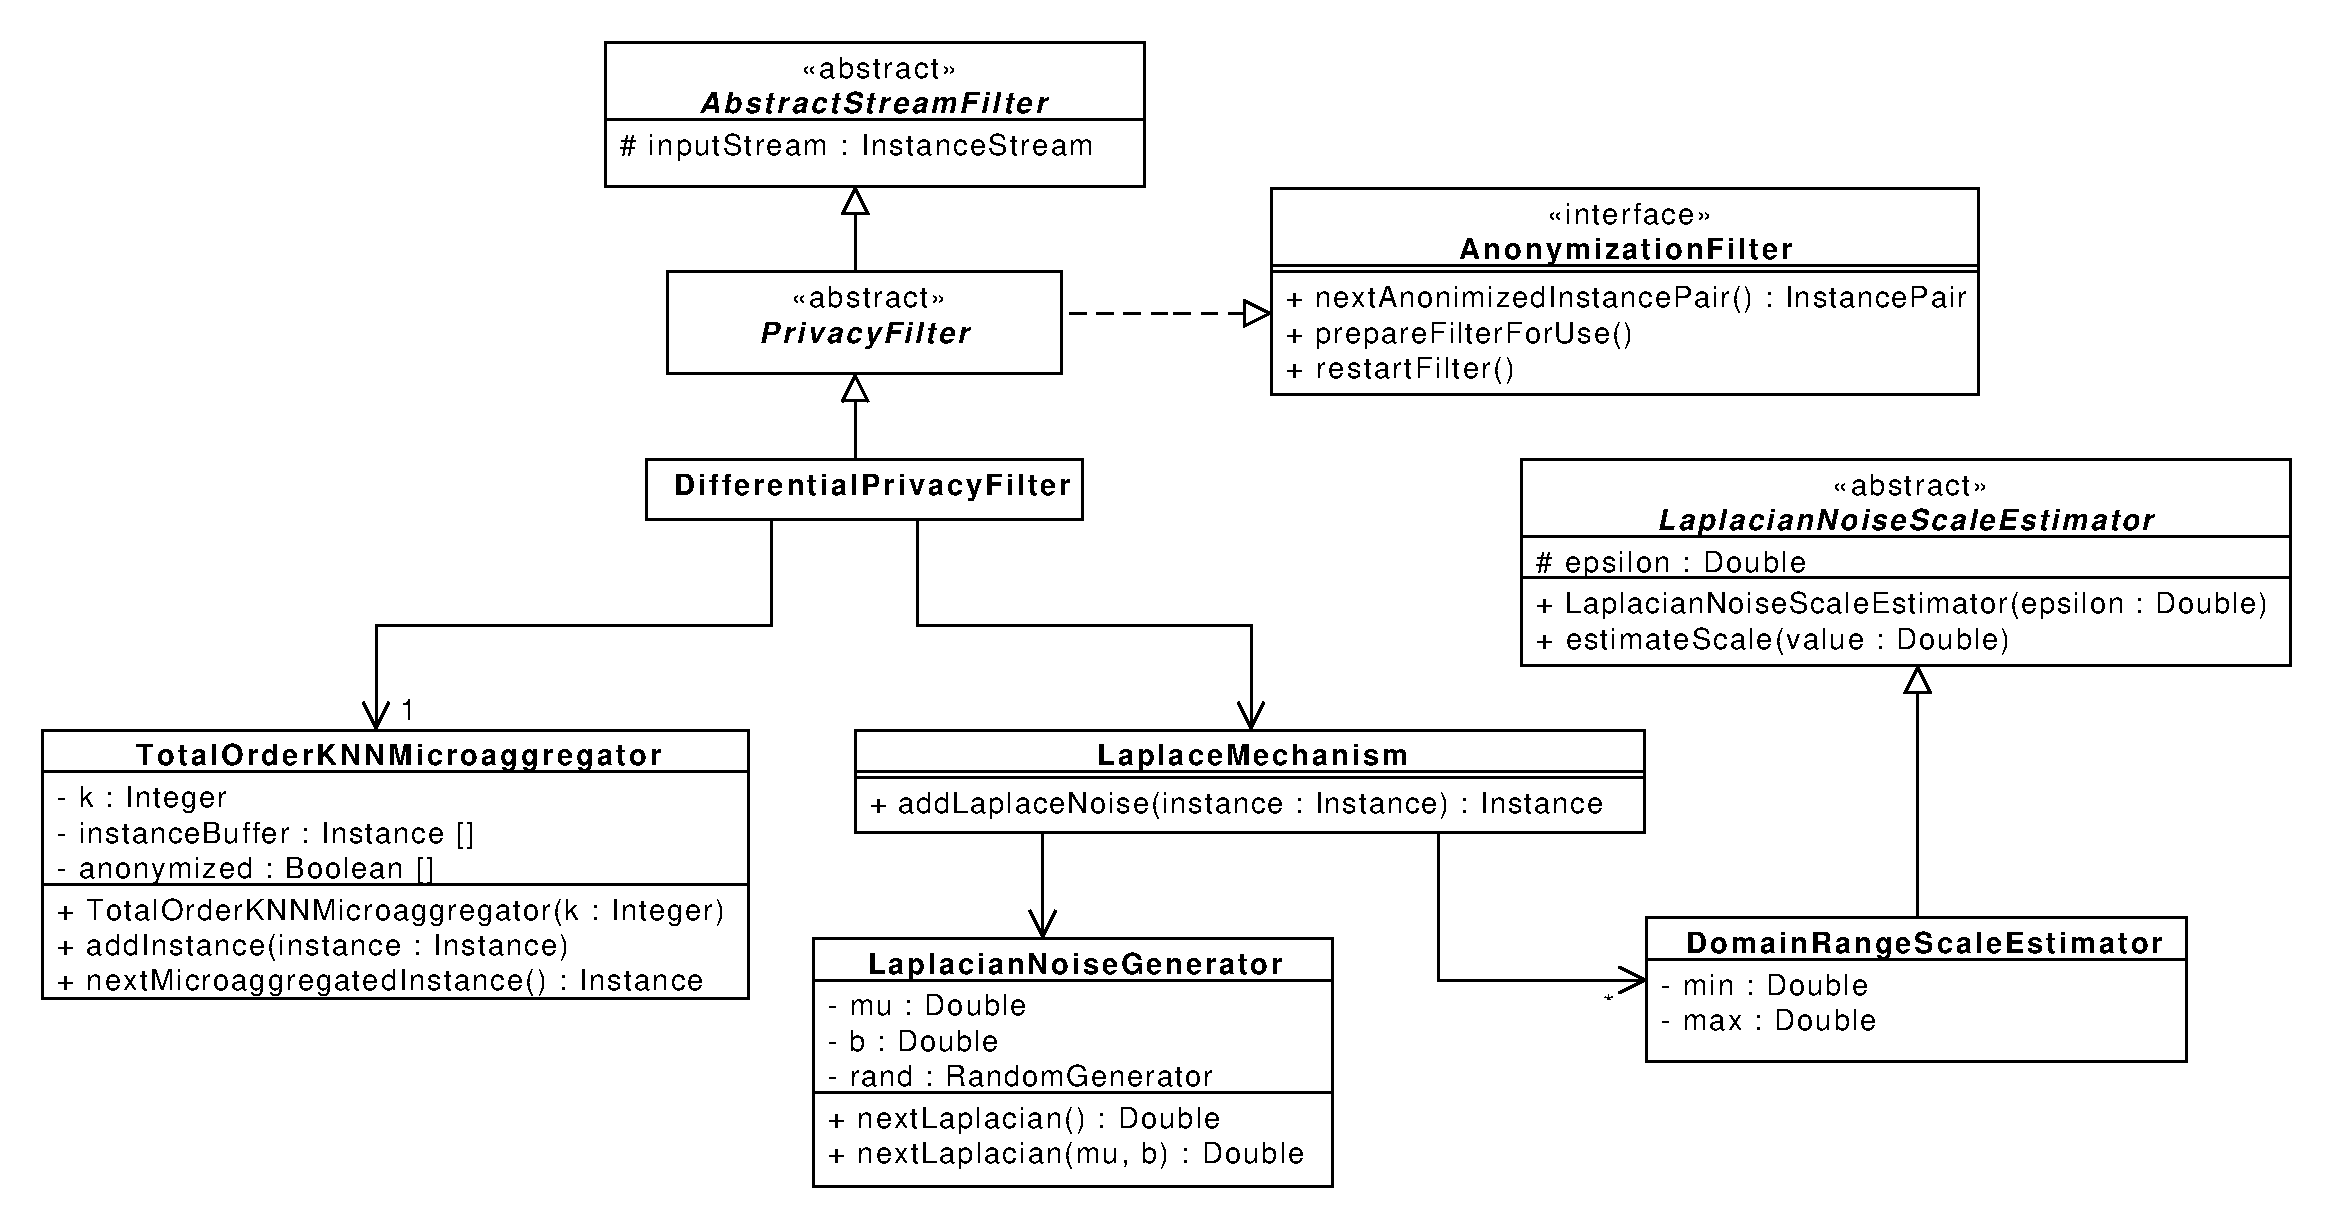
\includegraphics[width=1.0\linewidth]{figures/class_DifferentialPrivacyFilter.pdf}
	\caption[\texttt{DifferentialPrivacyFilter} class environment.]{\texttt{DifferentialPrivacyFilter} and the related classes and types it uses. Notice that the \texttt{LaplaceMechanism} uses many noise scale estimators, one for each attribute in the stream.}
	\label{fig:class-differential-privacy-filter}
\end{figure}

The adaptation of the insensitive microaggregation algorithm to a stream processing environment follows the same scheme presented for the \texttt{MicroAggregationFilter} (see~\sref{Implementation:Microaggregation:Design}), the only difference being the use of a \textit{reference} point in order to achieve a total ordering relation between the instances of the stream and, thus, fulfilling the insensitivity condition. The reference ``point'', denoted by $\mathcal{R}$, is incrementally\footnote{Remember that, in a stream processing environment, and more precisely, in the context of a \textit{buffered filter} (see~\sref{Implementation:BufferedFilter}), only a portion of the complete dataset (the stream) is visible to the algorithm at a given moment.} built as \textit{new} instances are processed by the filter, this is, it is updated independently of the clustering step, when a new instance is added to the buffer. The necessary modifications are presented in \alref{al:insensitive microaggregation}.

\begin{algorithm}[h]
\KwData{$W', A$ buffers and $\mathcal{R}$, the current reference point}
\KwResult{a \textit{cluster} $\mathcal{C}$ of $k$ instances}
\Begin{
	$\mathcal{C} \leftarrow \emptyset$\;
	$Q \leftarrow$ PriorityQueue$\langle$DistanceInstancePair$\rangle$()\;
	\For{$ x \in W', x \notin A $}{
		$d \leftarrow \mathrm{dist}(x,\mathcal{R})$\;
		$p \leftarrow$ DistanceInstancePair($d$, $x$)\;
		\eIf{$\vert Q \vert < k$}{
			$Q \leftarrow Q \cup p$\;
		}{
			\If{$p < Q$.peek().distance()}{
				$Q.poll()$\;
				$Q \leftarrow Q \cup p$\;
			}
		}
	}
	\For{$q \in Q$}{
		$\mathcal{C} \leftarrow \mathcal{C} \cup q.instance()$\;
	}
	\KwRet $\mathcal{C}$\;
}
\caption{KNN-based Insensitive Clustering\label{al:insensitive microaggregation}}
\end{algorithm}

The Laplace-distributed noise addition step of the mechanism is performed by a noise adder (called $\mathcal{L}$ in~\alref{al:laplace-mechanism}) that works in a very similar fashion to the \texttt{NoiseAdditionFilter}, with the addition of the scale parameter estimation, already discussed before. The complete description of the procedure is given in~\alref{al:laplace-noise-adder} and, finally, the generation of a random variable $\Lambda$ following a Laplace distribution is shown in the equation below:

\begin{equation}
\Lambda \sim Lap(\mu,b) \iff \Lambda = \mu - b~\mathrm{sgn}(U)~\ln(1-2\vert U \vert)
\end{equation}

where $U$ is another random variable drawn from a uniform distribution constrained to the $(-0.5,0.5]$ interval.

\begin{algorithm}
\KwData{an instance $x$ and a vector $B$ of scale estimators}
\KwResult{an anonymized instance $x'$}
\Begin{
	\For{$i \in \mathrm{attributes}(x)$}{
		$b \leftarrow B_i.estimate(x_i)$\;
		$x_i' \leftarrow x_i + \mathrm{Random}.laplace(0,b)$\;
	}
	\KwRet{$x'$}\;
}
\caption{Laplace Noise Adder\label{al:laplace-noise-adder}}
\end{algorithm}

\subsection{Summary}
\label{Implementation:DifferentialPrivacy:Summary}

The \texttt{DifferentialPrivacyFilter} class implements a microaggregation-based Laplace mechanism to achieve $\varepsilon$-differential privacy sanitization of released data.~\tref{table:differential-privacy-summary} summarizes the main properties of this SDC method.

\begin{table}[h]
	\centering
	\begin{tabular}{@{}ll@{}}
	\toprule
	\multicolumn{2}{l}{\textbf{DifferentialPrivacyFilter}}                             \\ \midrule
	\textbf{Parameters}   & $k$ (cluster size), $\varepsilon$ (differential privacy), $b$ (buffer size) \\
	\textbf{Type of data} & Numerical data only \\
	\textbf{Cost}         & $O(n \cdot b \cdot \mathrm{log}(k))$  \\ \bottomrule
	\end{tabular}
	\caption{\texttt{DifferentialPrivacyFilter} summary.}
	\label{table:differential-privacy-summary}
\end{table}